% Build this document with LuaTeX, a modern Unicode-aware LaTeX engine
% that uses system TTF and OTF font files.
% This is needed for the fontspec, microtype, and nolig packages.

\newcommand{\bodyfontsize}{10bp}
\newcommand{\bodybaselineskip}{12bp}

\RequirePackage[table]{xcolor}

% We're using KOMA Script to hand-tune footnotes and TOC appearance.
% It should be available in your texlive distribution,
% which is how most distros package LaTeX.
\documentclass[fontsize=10pt, oneside]{scrartcl}

% Margins: see http://practicaltypography.com/page-margins.html and
% http://practicaltypography.com/line-length.html
% We're aiming for 80-ish characters per line.
\usepackage[
    letterpaper,
    footnotesep=\bodybaselineskip,
    left=0.75in,right=0.75in,top=1in,bottom=1in,
]{geometry}

% Font specification.
\usepackage[no-math]{fontspec}
\usepackage[fleqn]{amsmath}

\usepackage[italic]{mathastext}

\usepackage{polyglossia}
\setdefaultlanguage[variant=american]{english}

\usepackage{microtype} % Font expansion, protrusion, and other goodness

% Disable ligatures across grapheme boundaries
% (see the package manual for details.)
\usepackage[english]{selnolig}

% Use symbols for footnotes, resetting each page
\usepackage[perpage,bottom,symbol*]{footmisc}

% Don't use a sans font for description labels.
\addtokomafont{descriptionlabel}{\rmfamily\mdseries}
\setkomafont{disposition}{\rmfamily}
\setkomafont{section}{\large\itshape}
\setkomafont{subsection}{\normalsize\itshape}
\renewcommand*\thesection{\upshape\arabic{section}}

\usepackage{enumitem}

% Custom footer
\usepackage{scrlayer-scrpage}
\setkomafont{pagefoot}{\sffamily\upshape}
\pagestyle{scrheadings}

\usepackage{minted} % Syntax highlighting via Pygments

\usepackage{graphicx}
\usepackage[font=footnotesize,justification=raggedright]{caption}

\usepackage{tikz} % Duck and cover.

\newcommand{\codesize}{\fontsize{\bodyfontsize}{\bodybaselineskip}}

% Syntax highlighting for Arm asm (minted doesn't do this well)
\usepackage{listings}
\lstset{
basicstyle=\ttfamily\codesize\selectfont,
keywordstyle=\color{darkGreen}\bfseries,
commentstyle=\textcolor[rgb]{0.25,0.50,0.50}
}
% listings definitions for Arm assembly.
% Get them from https://github.com/sysprog21/arm-assembler-latex-listings
\usepackage{lstlangarm} % See above

\usepackage{changepage} % For adjustwidth

\usepackage{metalogo} % for \LuaLaTeX

\newminted[ccode]{c}{
  baselinestretch=1,
  breaklines,
  breakafter=d,
}

\newminted[cppcode]{cpp}{
  baselinestretch=1,
  breaklines,
  breakafter=d,
}

\usemintedstyle{vs}

\NewDocumentCommand{\samplec}{oom}{%
  \IfNoValueTF{#1}%
  {%
    \inputminted[baselinestretch=1, breaklines, breakafter=d]{c}{#3}%
  }%
  {%
    \IfNoValueTF{#2}%
    {%
      \inputminted[baselinestretch=1, breaklines, breakafter=d, firstline=#1]{c}{#3}%
    }%
    {%
      \inputminted[baselinestretch=1, breaklines, breakafter=d, firstline=#1, lastline=#2]{c}{#3}%
    }%
  }%
}

\newminted[shcode]{bash}{
  baselinestretch=1.2,
  breaklines,
  breakafter=d,
}

\newmintinline[sh]{bash}{}
\newmintinline[cc]{c}{}
\newmintinline[cpp]{cpp}{}


\setlength\columnsep{2em}
%\setlength\parskip{0em}
\setlength\parindent{1.5em}

\title{Concurrency Primer\footnote{%
The original title was ``What every systems programmer should know about concurrency''.}
}
\author{Matt Kline and Ching-Chun (Jim) Huang}
\date{\today}

% Custom footer
% Hyperlinks
\usepackage[unicode,pdfusetitle]{hyperref}
\usepackage{xcolor}
\definecolor{darkGreen}{HTML}{008000}
\hypersetup{
    colorlinks=true, % Use colors
    linkcolor=violet, % Intra-doc links
    urlcolor=blue % URLs are blue
}

% Use \punckern to overlap periods, commas, and footnote markers
% for a tighter look.
% Care should be taken to not make it too tight - f" and the like can overlap
% if you're not careful.
\newcommand{\punckern}{\kern-0.4ex}
% For placing commas close to, or under, quotes they follow.
% We're programmers, and we blatantly disregard American typographical norms
% to put the quotes inside, but we can at least make it look a bit nicer.
\newcommand{\quotekern}{\kern-0.5ex}


% Create an unbreakable string of text in a monospaced font.
% Useful for `command --line --args`
\newcommand{\monobox}[1]{\mbox{\texttt{#1}}}

\newcommand{\keyword}[1]{\monobox{\color{darkGreen}#1}}

% C++ looks nicer if the ++ is in a monospace font and raised a bit.
% Also, use uppercase numbers to match the capital C.
\newcommand{\cplusplus}[1]{C\kern-0.1ex\raisebox{0.15ex}{\texttt{++}}}
\newcommand{\clang}[1]{C}
\newcommand{\csharp}{C\raisebox{0.25ex}{\#}}

\newcommand{\fig}[1]{Figure~\ref{#1}}

% Italicize new terms
\newcommand{\introduce}[1]{\textit{#1}}

\newcommand{\secref}[1]{\hyperref[#1]{\textsc{\S}\ref*{#1}}}

% See http://tex.stackexchange.com/a/68310
\makeatletter
\let\runauthor\@author
\let\rundate\@date
\let\runtitle\@title
\makeatother

% Spend a bit more time to get better word spacing.
% See http://tex.stackexchange.com/a/52855/92465
\emergencystretch=1em

\begin{document}
% Custom title instead of \maketitle
\begin{center}
\Large \runtitle
\bigskip

\large
\runauthor
\smallskip

\normalsize
\rundate
\end{center}
\bigskip

\begin{center}
\large \bfseries\itshape Abstract
\end{center}
\smallskip

\noindent
System programmers are acquainted with tools such as mutexes, semaphores, and condition variables.
However, the question remains: how do these tools work, and how do we write concurrent code in their absence?
For example, when working in an embedded environment beneath the operating system,
or when faced with hard time constraints that prohibit blocking.
Furthermore, since the compiler and hardware often combine to transform code into an unanticipated order,
how do multithreaded programs work? Concurrency is a complex and counterintuitive topic,
but let us endeavor to explore its fundamental principles.
\bigskip

\section{Background}
\label{background}

Modern computers execute multiple instruction streams concurrently.
On single-core systems, these streams alternate, sharing the \textsc{CPU} in brief time slices.
Multi-core systems, however, allow several streams to run in parallel.
These streams are known by various names such as processes, threads, tasks,
interrupt service routines (ISR), among others, yet many of the same principles govern them all.

Despite the development of numerous sophisticated abstractions by computer scientists,
these instruction streams—hereafter referred to as ``\emph{threads}'' for simplicity—primarily interact through shared state.
Proper functioning hinges on understanding the sequence in which threads read from and write to memory.
Consider a simple scenario where thread \textit{A} communicates an integer with other threads:
it writes the integer to a variable and then sets a flag, signaling other threads to read the newly stored value.
This operation could be conceptualized in code as follows:
\begin{ccode}
int v;
bool v_ready = false;

void threadA()
{
    // Write the value
    // and set its ready flag.
    v = 42;
    v_ready = true;
}
\end{ccode}

\begin{ccode}
void threadB()
{
    // Await a value change and read it.
    while (!v_ready) { /* wait */ }
    const int b_v = v;
    // Do something with b_v...
}
\end{ccode}
We must ensure that other threads only observe \textit{A}'s write to \cc|v_ready| \emph{after A's} write to \cc|v|.
If another thread can ``see'' \cc|v_ready| becoming true before observing \cc|v| becoming $42$,
this simple scheme will not work correctly.

One might assume it is straightforward to ensure this order,
yet the reality is often more complex.
Initially, any optimizing compiler will restructure your code to enhance performance on its target hardware.
The primary objective is to maintain the operational effect within \emph{the current thread},
allowing reads and writes to be rearranged to prevent pipeline stalls\footnote{%
Most \textsc{CPU} architectures execute segments of multiple instructions concurrently to improve throughput (refer to \fig{pipeline}).
A stall, or suspension of forward progress, occurs when an instruction awaits the outcome of a preceding one in the pipeline until the necessary result becomes available.} or to optimize data locality.\punckern\footnote{%
\textsc{RAM} accesses data not byte by byte, but in larger units known as \introduce{cache lines}.
Grouping frequently used variables on the same cache line means they are processed together,
significantly boosting performance. However, as discussed in \secref{false-sharing},
this strategy can lead to complications when cache lines are shared across cores.}

Variables may be allocated to the same memory location if their usage does not overlap.
Furthermore, calculations might be performed speculatively ahead of a branch decision and subsequently discarded if the branch prediction proves incorrect.\punckern\footnote{%
Profile-guided optimization (PGO) often employs this strategy.}
%(These sorts of optimizations  sometimes called the ``as-if'' rule in \cplusplus{}.)

Even without compiler alterations,
we would face challenges because our hardware complicates matters further!
Modern \textsc{CPU}s operate in a fashion far more complex than what traditional pipelined methods,
like those depicted in \fig{pipeline}, suggest.
They are equipped with multiple data paths tailored for various instruction types and schedulers that reorder and direct instructions through these paths.

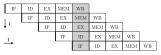
\includegraphics[keepaspectratio,width=0.7\linewidth]{images/pipeline}
\captionof{figure}{A traditional five-stage \textsc{CPU} pipeline with fetch, decode, execute, memory access, and write-back stages.
                   Modern designs are much more complicated, often reordering instructions on the fly.}
\label{pipeline}

It is quite common to form oversimplified views about memory operations.
Picturing a multi-core processor setup might lead us to envision a model similar to \fig{ideal-machine},
wherein each core alternately accesses and manipulates the system's memory.
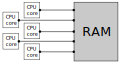
\includegraphics[keepaspectratio, width=0.8\linewidth]{ideal-machine}
\captionof{figure}{An idealized multi-core processor where cores
take turns accessing a single shared set of memory.}
\label{ideal-machine}

The reality is far from straightforward.
Although processor speeds have surged exponentially in recent decades,
\textsc{RAM} has struggled to match pace,
leading to a significant gap between the execution time of an instruction and the time required to fetch its data from memory.
To mitigate this, hardware designers have incorporated increasingly complex hierarchical caches directly onto the \textsc{CPU} die.
Additionally, each core often features a \introduce{store buffer} to manage pending writes while allowing further instructions to proceed.
Ensuring this memory system remains \introduce{coherent},
thus allowing writes made by one core to be observable by others even when utilizing different caches,
presents a significant challenge.

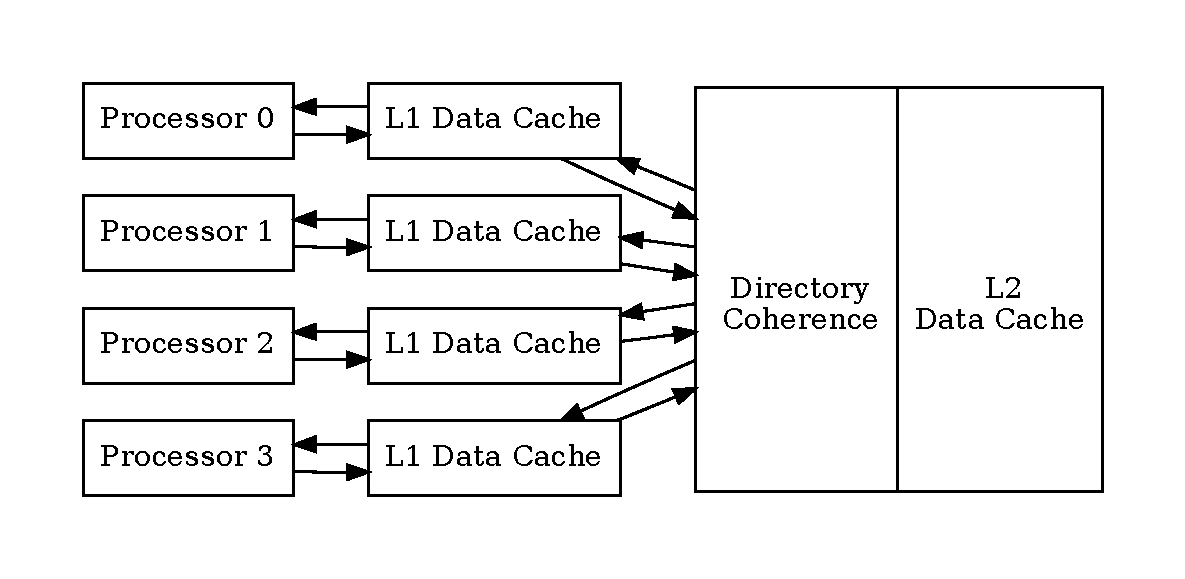
\includegraphics[keepaspectratio, width=0.8\linewidth]{images/mp-cache}
\captionof{figure}{A common memory hierarchy for modern multi-core processors}
\label{dunnington}

The myriad complexities within multithreaded programs on multi-core \textsc{CPU}s lead to a lack of a uniform concept of ``now''.
Establishing some semblance of order among threads requires a concerted effort involving the hardware,
compiler, programming language, and your application.
Let's delve into our options and the tools necessary for this endeavor.

\section{Enforcing law and order}
\label{seqcst}

Establishing order in multithreaded programs varies across different \textsc{CPU} architectures.
For years, systems languages like \clang{} and \cplusplus{} lacked built-in concurrency mechanisms,
compelling developers to rely on assembly or compiler-specific extensions.
This gap was bridged in 2011 when the \textsc{ISO} standards for both languages introduced synchronization tools.
Provided these tools are used correctly,
the compiler ensures that neither its optimization processes nor the \textsc{CPU} will perform reorderings that could lead to data races.\punckern\footnote{%
The ISO~\clang{11} standard adopted its concurrency features,
almost directly, from the \cplusplus{11} standard.
Thus, the functionalities discussed should be the same in both languages,
with some minor syntactical differences favoring \cplusplus{} for clarity.
}

To ensure our earlier example functions as intended,
the ``ready'' flag must utilize an \introduce{atomic type}.
\begin{ccode}
#include <stdatomic.h>
int v = 0;
atomic_bool v_ready = false;

void *threadA()
{
    v = 42;
    v_ready = true;
}
\end{ccode}
\begin{ccode}
int b_v;

void *threadB()
{
    while(!v_ready) { /* wait */ }
    b_v = v;
    /* Do something */
}
\end{ccode}
The \clang{} and \cplusplus{} standard libraries define a series of these types in \cc|<stdatomic.h>| and \cpp|<atomic>|,
respectively.
They look and act just like the integer types they mirror (e.g., \monobox{bool}~\textrightarrow~\monobox{atomic\_bool},
\monobox{int}~\textrightarrow~\monobox{atomic\_int}, etc.),
but the compiler ensures that other variables' loads and stores are not reordered around theirs.

Informally, we can think of atomic variables as rendezvous points for threads.
By making \monobox{v\_ready} atomic,
\monobox{v = 42}\, is now guaranteed to happen before \monobox{v\_ready = true}\, in thread~\textit{A},
just as \monobox{b\_v = v}\, must happen after reading \monobox{v\_ready}\,
in thread~\textit{B}.
Formally, atomic types establish a \textit{single total modification order} where,
``[\ldots] the result of any execution is the same as if the reads and writes occurred in some order, and the operations of each individual processor appear in this sequence in the order specified by its program.''
This model, defined by Leslie Lamport in 1979,
is called \introduce{sequential consistency}.

Notice that using atomic variables as an lvalue expression, such as \monobox{v\_ready = true} and \monobox{while(!v\_ready)}, is a convenient alternative to explicitly using \monobox{atomic\_load} or \monobox{atomic\_store}. 
Lvalue-to-rvalue conversion (which models a memory read from an atomic location to a CPU register) strips atomicity along with other qualifiers. 

\section{Atomicity}
\label{atomicity}
But order is only one of the vital ingredients for inter-thread communication.
The other is what atomic types are named for: atomicity.
Something is \introduce{atomic} if it can not be divided into smaller parts.
If threads do not use atomic reads and writes to share data, we are still in trouble.

Consider a program with two threads.
One thread processes a list of files, incrementing a counter each time it finishes working on one.
The other thread handles the user interface, periodically reading the counter to update a progress bar.
If that counter is a 64-bit integer, we can not access it atomically on 32-bit machines,
since we need two loads or stores to read or write the entire value.
If we are particularly unlucky, the first thread could be halfway through writing the counter when the second thread reads it,
receiving garbage.
These unfortunate occasions are called \introduce{torn reads and writes}.

If reads and writes to the counter are atomic, however, our problem disappears.
We can see that, compared to the difficulties of establishing the right order,
atomicity is fairly straightforward:
just make sure that any variables used for thread synchronization
are no larger than the \textsc{CPU} word size.

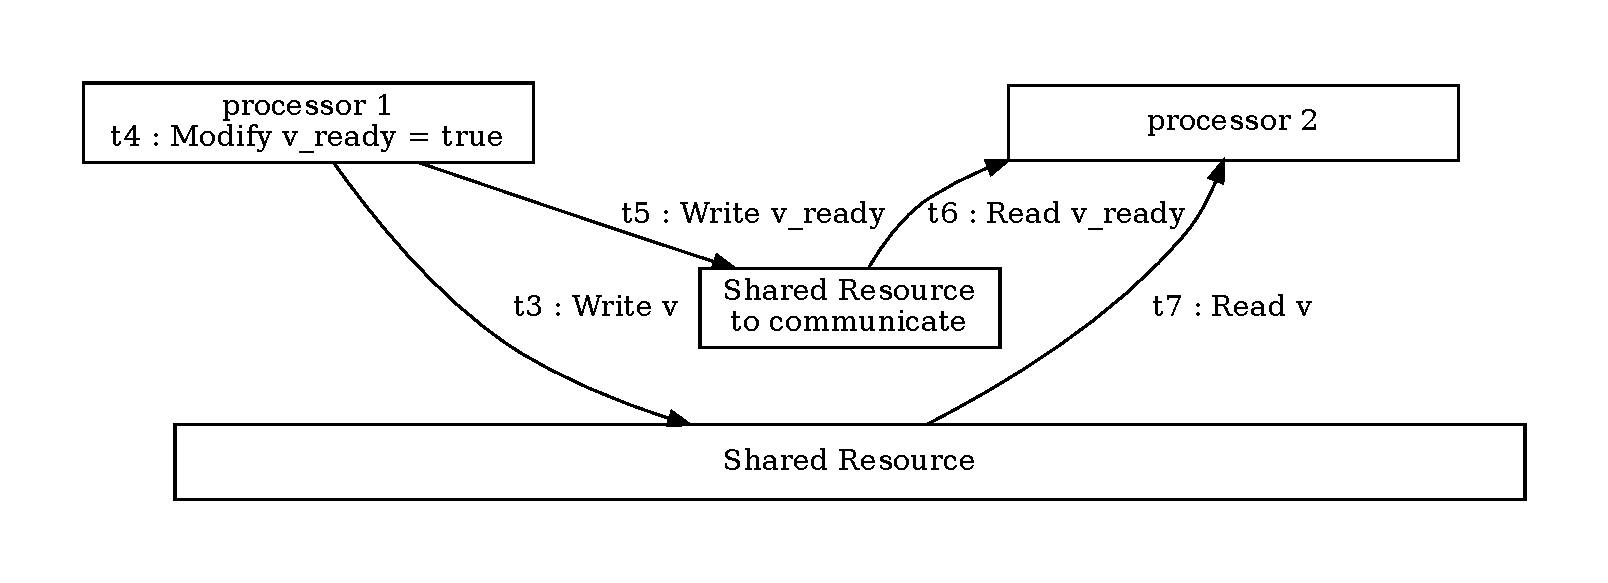
\includegraphics[keepaspectratio, width=0.8\linewidth]{images/atomicity}
\captionof{figure}{A flowchart depicting how two concurrent programs communicate and coordinate through a shared resource to achieve a goal, accessing the shared resource.}
\label{atomicity}

Summary of concepts from the first three sections, as shown in \fig{atomicity}.
In \secref{background}, we observe the importance of maintaining the correct order of operations: t3 \to t4 \to t5 \to t6 \to t7, so that two concurrent programs can function as expected.
In \secref{seqcst}, we see how two concurrent programs communicate to guarantee the order of operations: t5 \to t6.
In \secref{atomicity}, we understand that certain operations must be treated as a single atomic step to ensure the order of operations: t3 \to t4 \to t5 and the order of operations: t6 \to t7.

\section{Arbitrarily-sized ``atomic'' types}

Along with \cc|atomic_int| and friends,
\cplusplus{} provides the template \cpp|std::atomic<T>| for defining arbitrary atomic types.
\clang{}, lacking a similar language feature but wanting to provide the same functionality,
added an \keyword{\_Atomic} keyword.
If \texttt{T} is larger than the machine's word size,
the compiler and the language runtime automatically surround the variable's reads and writes with locks.
If you want to make sure this is not happening,\punckern\footnote{%
\ldots which is most of the time,
since we are usually using atomic operations to avoid locks in the first place.}
you can check with:
\begin{cppcode}
std::atomic<Foo> bar;
ASSERT(bar.is_lock_free());
\end{cppcode}
In most cases,\punckern\footnote{%
The language standards permit atomic types to be \emph{sometimes} lock-free.
This might be necessary for architectures that do not guarantee atomicity for unaligned reads and writes.}
this information is known at compile time.
Consequently, \cplusplus{17} added \cpp|is_always_lock_free|:
\begin{cppcode}
static_assert(std::atomic<Foo>::is_always_lock_free);
\end{cppcode}

\section{Read-modify-write}
\label{rmw}

So far we have introduced the importance of order and atomicity.
The latter ensures that no other operations on the target object success until the executing operation has finished.
This also establishes ordering between operations, as no operations can occur concurrently.
For two operations, A and B, either A happens before B or B happens before A.
As in \secref{seqcst}, a local order of other operations associated to the an atomic object is given as well, with \introduce{sequential consistency} as default consistency level.
Since happens before relation is transitive, just like $>$ and $<$, a global order is established by combining local order and inter-thread order provided by atomic objects. 

Atomic loads and stores are all well and good when we don't need to consider the previous state of atomic variables.
But sometimes we need to read a value, modify it,
and write it back as a single atomic step.
That is, the modification is based on the previous state that is visible for reading, and the result is then written back.
A complete \introduce{read-modify-write} operation is performed atomically to ensure visibility to subsequent operations.

There are a few common \introduce{read-modify-write} (\textsc{RMW}) operations.
In \cplusplus{}, they are represented as member functions of \cpp|std::atomic<T>|.
In \clang{}, they are freestanding functions.

Following example code is a simplify implementation of thread pool to demonstrate the use of \clang{}11 atomic library.

\inputminted{c}{./examples/rmw_example.c}

Compile the code with \monobox{gcc rmw\_example.c -o rmw\_example -Wall -Wextra -std=c11 -pthread} and execute the program.
A thread pool has three states: idle, cancelled and running. 
It is initialized with \monobox{N\_THREADS} (default 8) of threads. 
\monobox{N\_JOBS} (default 16) of jobs are added, and the pool is then set to running. 
A job is simply echoing its job ID.
\monobox{sleep(1)} is used to ensure that the second batch of jobs is added after the first batch is finished; otherwise, jobs may not be consumed as expected.
Thread pool is then destroyed right after starting running.
Possible stdout of the program is:
\begin{ccode}
Hello from job 5
Hello from job 8
Hello from job 9
Hello from job 10
Hello from job 11
Hello from job 12
Hello from job 13
Hello from job 14
Hello from job 15
Hello from job 3
Hello from job 1
Hello from job 6
Hello from job 4
Hello from job 7
Hello from job 2
Hello from job 0
Hello from job 0
Hello from job 1
Hello from job 3
Hello from job 2
Thread pool cancelled with jobs still running.
\end{ccode}

\subsection{Exchange}
\label{exchange}

The simplest atomic \textsc{RMW} operation is an \introduce{exchange}:
the current value is read and replaced with a new one.
In function \monobox{thread\_pool\_destroy}, \monobox{atomic\_exchange(\&thrd\_pool->state, cancelled)} reads current state and replaces it with "cancelled". A warning message is printed if the pool is destroyed when still running. 
If the exchange is not performed atomically, we may initially get the state as "running". Subsequently, a thread could set the state to "cancelled" after finishing the last one, resulting in a false warning.

\subsection{Test and set}

\introduce{Test-and-set} works on a Boolean value:
we read it, set it to \cpp|true|, and provide the value it held beforehand.
\clang{} and \cplusplus{} offer a type dedicated to this purpose, called \monobox{atomic\_flag}.
The value of the flag is indeterminate until initialized with \monobox{ATOMIC\_FLAG\_INIT} macro.
A thread pool has a \monobox{atomic\_flag} indicating it's initialized or not. The flag ensures initialization is thread-safe, preventing a pool from being reinitialized.
Function \monobox{thread\_pool\_init} sets the flag with \monobox{atomic\_flag\_test\_and\_set(\&thrd\_pool->initialezed)} first.
If the return value is \monobox{true}, initialization is not performed again.
Function \monobox{thread\_pool\_destroy} clears the flag with \monobox{atomic\_flag\_clear(\&thrd\_pool->initialezed)} after destroying everything.

\subsection{Fetch and…}

We can also read a value,
perform a simple operation on it (such as addition, subtraction,
or bitwise \textsc{AND}, \textsc{OR}, \textsc{XOR}) and return its previous value,
all as part of a single atomic operation.
In the function \monobox{thread\_pool\_destroy}, \monobox{atomic\_fetch\_and} is utilized as a means to set the state to idle. 
Yet, in this case, it is not necessary, as the pool needs to be reinitialized for further use regardless.
Its return value could be further utilized, for instance, to report the previous state and perform additional actions.

\subsection{Compare and swap}
\label{cas}

Finally, we have \introduce{compare-and-swap} (\textsc{CAS}),
sometimes called \introduce{compare-and-exchange}.
It allows us to conditionally exchange a value \emph{if} its previous value matches some expected one.
In \clang{} and \cplusplus{}, \textsc{CAS} resembles the following,
if it were executed atomically:
\begin{ccode}
/* A is an atomic type. C is the non-atomic type corresponding to A */
bool atomic_compare_exchange_strong(A* obj, C* expected, C desired)
{
    if (memcmp(obj, expected, sizeof(*object)) == 0) {
        memcpy(obj, &desired, sizeof(*object));
        return true;
    } else {
        memcpy(expected, obj, sizeof(*object));
        return false;
    }
}
\end{ccode}

\begin{samepage}
\noindent The \cpp|_strong| suffix may leave you wondering if there is a corresponding ``weak'' \textsc{CAS}.
Indeed, there is. However, we will delve into that topic later in \secref{spurious-llsc-failures}.
\end{samepage}

Once threads are created in the thread pool as workers, they will continuously search for jobs to do.
Jobs are taken from the tail of job queue.
To claim a job without it being taken by another worker halfway through, we need to atomically change the pointer to the last job. Otherwise the last job is under races.
The while loop in function \monobox{worker},
\begin{ccode}
while (!atomic_compare_exchange_strong(&thrd_pool->head->prev, &job,
                                       job->prev)) {
}
\end{ccode}
, keeps trying to claim the job atomically until success.

Built-in post increment and decrement operators and compound assignment on atomic objects, such as \monobox{++} and \monobox{+=}, are read-modify-write atomic operations with total sequentially consistent ordering as well. 
They behave equivalently to a \cc|do while| loop. See \clang{}11 standard 6.5.2.4 and 6.5.16.2 for more details.

What if claiming a job, which updates \cc|thrd_pool->head->prev|, is not done atomically?
Let's remove the atomicity of claiming a job and use thread sanitizer to detect races.
Thread sanitizer is one of the sanitizers provided by \introduce{gcc} and \introduce{clang} to detect data races. 
Data races are undefined behavior in \clang{}11 and \cplusplus{}11. 
Thread sanitizer inserts runtime code into the target program to track memory accesses. 
When races occur during execution, warning messages are printed.
To enable this, add \monobox{-fsanitize=thread -g} to compiler flags.
The following diff patch removes the atomicity of claiming a job and uses pthread instead of \clang{}11 thread, because thread sanitizer currently hasn't support \clang{}11 thread yet. 
Save diff as \monobox{racer.diff} and patch the example code by \monobox{\$ patch rmw\_example.c race.diff}.

\inputminted{diff}{./examples/racer.diff}

After compiling and running the example, you will see warning messages printed and same job IDs got echoed repeatly. 
The top two sections of a warning message indicate which two threads executed which function causing the data race.
The bottom two sections indicate how these two threads were created.
If the race occurred on a heap block, a third section would appear indicating how the block was allocated.
At the end of a warning message, a summary indicates the type of race and where it occurred.
You'll see that two lines of code, which claim a job, are highlighted as causing a data race on \cc|thrd_pool->head|.

You may notice that there is another part of the code causing races. 
While some workers were echoing ID, others were attempting to free the job, resulting in heap-use-after-free and data races.
This occurred when two workers claimed the same job, as the claiming process was not atomic.
But even when jobs were claimed atomically, this still can occur.
This is a defect of the example code.
Jobs in the example are dynamically allocated. They are freed after worker finishes each job. 
However, this situation may lead to dangling pointers for workers that are still holding and attempting to claim the job. 
If jobs are intended to be dynamically allocated, then safe memory reclamation should be implemented for such shared objects.
RCU, hazard pointer and reference counting are major ways of solving this problem.

\subsection{Further improvements}
At the beginning of \secref{rmw}, we described how a global total order is established by combining local order and inter-thread order imposed by atomic objects. 
But should every object, including non-atomic ones, participate in a single global order established by atomic objects?
\introduce{Sequential consistency} solves the ordering problem in in \secref{seqcst}, but it may force too much ordering, as some normal operations may not require it.
Without specifying, atomic operations in \clang{}11 atomic library use \monobox{memory\_order\_seq\_cst} as default memory order. Operations post-fix with \monobox{\_explicit} accept an additional argument to specify which memory order to use.
How to leverage memory orders to optimize performance will be covered later in \secref{lock-example}.

You may have noticed that there is padding after \monobox{\_Atomic(job\_t *) prev} in \monobox{struct idle\_job} in the example.
It is used for preventing \introduce{false sharing} in a cache line.
Further discussion on cache effects and false sharing is provided in \secref{false-sharing}.

\section{Atomic operations as building blocks}

Atomic loads, stores, and \textsc{RMW} operations are the building blocks for every single concurrency tool.
It is useful to split those tools into two camps:
\introduce{blocking} and \introduce{lockless}.

Blocking synchronization methods are generally easier to understand,
but they can cause threads to pause for unpredictable durations.
Take a mutex as an example:
it requires threads to access shared data sequentially.
If a thread locks the mutex and another attempts to lock it too,
the second thread must wait, or \introduce{block},
until the first one unlocks it, regardless of the wait time.
Additionally, blocking mechanisms are prone to \introduce{deadlock} and \introduce{livelock},
issues that lead to the system becoming immobilized as threads perpetually wait on each other.

In contrast, lockless synchronization methods ensure that the program is always making forward progress.
These are \introduce{non-blocking} since no thread can cause another to wait indefinitely.
Consider a program that streams audio,
or an embedded system where a sensor triggers an interrupt service routine (\textsc{ISR}) when new data arrives.
We want lock-free algorithms and data structures in these situations,
since blocking could break them.
(In the first case, the user's audio will begin to stutter if sound data is not provided at the bitrate it is consumed.
In the second, subsequent sensor inputs could be missed if the \textsc{isr} does not complete as quickly as possible.)

% FIXME: remove this hack
% LaTeX provides 9 symbols when using symbol option, therefore it produces an error if we count higher.
\setcounter{footnote}{0}
Lockless algorithms are not inherently superior or quicker than blocking ones;
they serve different purposes with their own design philosophies.
Additionally, the mere use of atomic operations does not render algorithms lock-free.
For example, basic spinlock is still considered a blocking algorithm even though it eschews \textsc{OS}-specific syscalls for making the blocked thread sleep.
Putting a blocked thread to sleep is often an optimization,
allowing the operating system's scheduler to allocate \textsc{CPU} resources to active threads until the blocked one is revived.
Some concurrency libraries even introduce hybrid locks that combine brief spinning with sleeping to balance \textsc{CPU} usage and context-switching overheads.

Both blocking and lockless approaches have their place in software development.
When performance is a key consideration, it is crucial to profile your application.
The performance impact varies with numerous factors, such as thread count and \textsc{CPU} architecture specifics.
Balancing complexity and performance is essential in concurrency, a domain fraught with challenges.

\section{Sequential consistency on weakly-ordered hardware}

Different hardware architectures offer distinct memory models or \introduce{memory models}.
For instance, x64 architecture\punckern\footnote{%
Also known as x86-64, x64 is a 64-bit extension of the x86 instruction set, officially unveiled in 1999.
This extension heralded the introduction of two novel operation modes:
64-bit mode for leveraging the full potential of 64-bit processing and compatibility mode for maintaining support for 32-bit applications.
Initially developed by AMD and publicly released in 2000, the x64 architecture has since been adopted by Intel and VIA,
signaling a unified industry shift towards 64-bit computing.
This wide adoption marked the effective obsolescence of the Intel Itanium architecture (IA-64),
despite its initial design to supersede the x86 architecture.
} is known to be \introduce{strongly-ordered},
generally ensuring a global sequence for loads and stores in most scenarios.
Conversely, architectures like \textsc{Arm} are considered \introduce{weakly-ordered},
meaning one should not expect loads and stores to follow the program sequence without explicit instructions to the \textsc{CPU}.
These instructions, known as \introduce{memory barriers}, are essential to prevent the reordering of these operations.

It is helpful to see how atomic operations work in a weakly-ordered system,
both to understand what's happening in hardware,
and to see why the \clang{} and \cplusplus{} concurrency models were designed as they were.\punckern\footnote{%
It is worth noting that the concepts we discuss here are not specific to \clang{} and \cplusplus{}.
Other systems programming languages like D and Rust have converged on similar models.}
Let's examine \textsc{Arm}, since it is both popular and straightforward.
Consider the simplest atomic operations: loads and stores.
Given some \cc|atomic_int foo|,
\newline
% Shield your eyes.
% Essentially,
% 1. On the left, place getFoo() and setFoo() functions.
% 2. On the right, place the assembly they are compiled to.
% 3. In the middle, place an arrow for each (futzing with height a bit)
%    with the text "becomes" over it.
\begin{minipage}{0.35\linewidth}
\begin{ccode}
int getFoo()
{
    return foo;
}
\end{ccode}
\end{minipage}
\raisebox{-1ex}{
\begin{tikzpicture}
\draw [->, line width=1pt] (0, 0) -- node[above]{\itshape becomes} (0.17\linewidth, 0);
\end{tikzpicture}
}
\begin{minipage}{0.43\linewidth}
\begin{lstlisting}[language={[ARM]Assembler}]
getFoo:
  ldr r3, <&foo>
  dmb
  ldr r0, [r3, #0]
  dmb
  bx lr
\end{lstlisting}
\end{minipage}
%Similarly,
\begin{minipage}{0.35\linewidth}
\begin{ccode}
void setFoo(int i)
{
    foo = i;
}
\end{ccode}
\end{minipage}
\raisebox{-1ex}{
\begin{tikzpicture}
\draw [->, line width=1pt] (0, 0) -- node[above]{\itshape becomes} (0.17\linewidth, 0);
\end{tikzpicture}
}
\begin{minipage}{0.43\linewidth}
\begin{lstlisting}[language={[ARM]Assembler}]
setFoo:
  ldr r3, <&foo>
  dmb
  str r0, [r3, #0]
  dmb
  bx lr
\end{lstlisting}
\end{minipage}
We load the address of our atomic variable into a scratch register (\texttt{r3}),
place our load or store operation between memory barriers (\keyword{dmb}), and then proceed.
These barriers ensure sequential consistency:
the first barrier guarantees that previous reads and writes are not reordered to follow our operation,
and the second ensures that future reads and writes are not reordered to precede it.

\section{Implementing atomic read-modify-write operations with LL/SC instructions}

Like many \textsc{RISC}\footnote{%
\introduce{Reduced instruction set computer}, in contrast to a \introduce{complex instruction set computer} (\textsc{CISC}) architecture like x64.
} architectures, \textsc{Arm} does not have dedicated \textsc{RMW} instructions.
Given that the processor may switch contexts to another thread at any moment,
constructing \textsc{RMW} operations from standard loads and stores is not feasible.
Special instructions are required instead: \introduce{load-link} and \introduce{store-conditional} (\textsc{LL/SC}).
These instructions are complementary:
load-link performs a read operation from an address, similar to any load,
but it also signals the processor to watch that address.
Store-conditional executes a write operation only if no other writes have occurred at that address since its paired load-link.
This mechanism is illustrated through an atomic fetch and add example.

On \textsc{Arm},
\begin{ccode}
void incFoo() { ++foo; }
\end{ccode}
compiles to:
\begin{lstlisting}[language={[ARM]Assembler}]
incFoo:
  ldr r3, <&foo>
  dmb
loop:
  ldrex r2, [r3] // LL foo
  adds r2, r2, #1 // Increment
  strex r1, r2, [r3] // SC
  cmp r1, #0 // Check the SC result.
  bne loop // Loop if the SC failed.
  dmb
  bx lr
\end{lstlisting}
We \textsc{LL} the current value, add one, and immediately try to store it back with a \textsc{SC}.
If that fails, another thread may have written to \texttt{foo} since our \textsc{LL}, so we try again.
In this way, at least one thread is always making forward progress in atomically modifying \texttt{foo},
even if several are attempting to do so at once.\punckern\footnote{%
\ldots though generally,
we want to avoid cases where multiple threads are vying for the same variable for any significant amount of time.}

\subsection{Spurious LL/SC failures}
\label{spurious-llsc-failures}

It is impractical for \textsc{CPU} hardware to track load-linked addresses for each byte within a system due to the immense resource requirements.
To mitigate this, many processors monitor these operations at a broader scale, like the cache line level.
Consequently, a \textsc{SC} operation may fail if any part of the monitored block is written to,
not just the specific address that was load-linked.

This limitation poses a particular challenge for operations like compare and swap,
highlighting the essential purpose of \monobox{compare\_exchange\_weak}.
Consider, for example, the task of atomically multiplying a value without an architecture-specific atomic read-multiply-write instruction.
\begin{cppcode}
void atomicMultiply(int by)
{
    int expected = foo;
    // Which CAS should we use?
    while (!foo.compare_exchange_?(expected, expected * by)) {
        // Empty loop.
        // (On failure, expected is updated with foo's most recent value.)
    }
}
\end{cppcode}
Many lockless algorithms use \textsc{CAS} loops like this to atomically update a variable when calculating its new value is not atomic.
They:
\begin{enumerate}
  \item Read the variable.
  \item Perform some (non-atomic) operation on its value.
  \item \textsc{CAS} the new value with the previous one.
  \item If the \textsc{CAS} failed, another thread beat us to the punch, so try again.
\end{enumerate}
If we use \monobox{compare\_exchange\_strong} for this family of algorithms,
the compiler must emit nested loops:
an inner one to protect us from spurious \textsc{SC} failures,
and an outer one which repeatedly performs our operation until no other thread has interrupted us.
But unlike the \monobox{\_strong} version,
a weak \textsc{CAS} is allowed to fail spuriously, just like the \textsc{LL/SC} mechanism that implements it.
So, with \monobox{compare\_exchange\_weak},
the compiler is free to generate a single loop,
since we do not care about the difference between retries from spurious \textsc{SC} failures and retries caused by another thread modifying our variable.

\section{Do we always need sequentially consistent operations?}
\label{lock-example}

All of our examples so far have been sequentially consistent to prevent reorderings that break our code.
We have also seen how weakly-ordered architectures like \textsc{Arm} use memory barriers to create sequential consistency.
But as you might expect,
these barriers can have a noticeable impact on performance.
After all,
they inhibit optimizations that your compiler and hardware would otherwise make.

What if we could avoid some of this slowdown?
Consider a simple case like spinlock.
\begin{ccode}
atomic_flag af = ATOMIC_FLAG_INIT;

void lock()
{
    while (atomic_flag_test_and_set(&af)) { /* wait */ }
}

void unlock() { atomic_flag_clear(&af); }
\end{ccode}
Between the \cc|lock()| and \cc|unlock()| calls,
we have a \introduce{critical section} where we can safely modify shared state protected by the lock.
Outside this critical section,
we only read and write to things that are not shared with other threads.
\begin{cppcode}
deepThought.calculate(); // non-shared

lock(); // Lock; critical section begins
sharedState.subject = "Life, the universe and everything";
sharedState.answer = 42;
unlock(); // Unlock; critical section ends

demolishEarth(vogons); // non-shared
\end{cppcode}

It is vital that reads and writes to shared memory do not move outside the critical section.
But the opposite is not true!
The compiler and hardware could move as much as they want \emph{into} the critical section without causing any trouble.
We have no problem with the following if it is somehow faster:
\begin{cppcode}
lock(); // Lock; critical section begins
deepThought.calculate(); // non-shared
sharedState.subject = "Life, the universe and everything";
sharedState.answer = 42;
demolishEarth(vogons); // non-shared
unlock(); // Unlock; critical section ends
\end{cppcode}
So, how do we tell the compiler as much?

\section{Memory orderings}

By default, all atomic operations, including loads, stores, and various forms of \textsc{RMW},
are considered sequentially consistent.
However, this is just one among many possible orderings.
We will explore each of these orderings in detail.
A comprehensive list, as well as the corresponding enumerations used by the \clang{} and \cplusplus{} \textsc{API}, can be found here:
\begin{itemize}
\item Sequentially Consistent (\monobox{memory\_order\_seq\_cst})
\item Acquire (\monobox{memory\_order\_acquire})
\item Release (\monobox{memory\_order\_release})
\item Relaxed (\monobox{memory\_order\_relaxed})
\item Acquire-Release (\monobox{memory\_order\_acq\_rel})
\item Consume (\monobox{memory\_order\_consume})
\end{itemize}
To pick an ordering,
you provide it as an optional argument that we have slyly failed to mention so far:\footnote{%
In \clang{}, separate functions are defined for cases where specifying an ordering is necessary.
\cc|exchange()| becomes \cc|exchange_explicit()|, a \textsc{CAS}
becomes \cc|compare_exchange_strong_explicit()|, and so on.}
\begin{cppcode}
void lock()
{
    while (af.test_and_set(memory_order_acquire)) { /* wait */ }
}

void unlock()
{
    af.clear(memory_order_release);
}
\end{cppcode}
Non-sequentially consistent loads and stores also use member functions of \cpp|std::atomic<>|:
\begin{cppcode}
int i = foo.load(memory_order_acquire);
\end{cppcode}
Compare-and-swap operations are a bit odd in that they have \emph{two} orderings: one for when the \textsc{CAS} succeeds, and one for when it fails:
\begin{cppcode}
while (!foo.compare_exchange_weak(
    expected, expected * by,
    memory_order_seq_cst, // On success
    memory_order_relaxed)) // On failure
    { /* empty loop */ }
\end{cppcode}

With the syntax out of the way,
let's look at what these orderings are and how we can use them.
As it turns out, almost all of the examples we have seen so far do not actually need sequentially consistent operations.

\subsection{Acquire and release}

We have just examined the acquire and release operations in the context of the lock example from \secref{lock-example}.
You can think of them as ``one-way'' barriers: an acquire operation permits other reads and writes to move past it,
but only in a $before \to after$ direction.
A release works the opposite manner, allowing actions to move in an $after \to before$ direction.
On \textsc{Arm} and other weakly-ordered architectures, this enables us to eliminate one of the memory barriers in each operation,
such that

 \begin{cppcode}
int acquireFoo()
{
    return foo.load(memory_order_acquire);
}

void releaseFoo(int i)
{
    foo.store(i, memory_order_release);
}
\end{cppcode}
become:
\begin{minipage}{0.45\linewidth}
\begin{lstlisting}[language={[ARM]Assembler}]
acquireFoo:
  ldr r3, <&foo>
  ldr r0, [r3, #0]
  dmb
  bx lr
\end{lstlisting}
\end{minipage}
\begin{minipage}{0.45\linewidth}
\begin{lstlisting}[language={[ARM]Assembler}]
releaseFoo:
  ldr r3, <&foo>
  dmb
  str r0, [r3, #0]
  bx lr
\end{lstlisting}
\end{minipage}

Together, these provide $writer \to reader$ synchronization:
if thread \textit{W} stores a value with release semantics,
and thread \textit{R} loads that value with acquire semantics,
then all writes made by \textit{W} before its store-release are observable to \textit{R} after its load-acquire.
If this sounds familiar, it is exactly what we were trying to achieve in
\secref{background} and \secref{seqcst}:
\begin{cppcode}
int v;
std::atomic_bool v_ready(false);

void threadA()
{
    v = 42;
    v_ready.store(true, memory_order_release);
}

void threadB()
{
    while (!v_ready.load(memory_order_acquire)) {
        // wait
    }
    assert(v == 42); // Must be true
}
\end{cppcode}

\subsection{Relaxed}
Relaxed atomic operations are useful for variables shared between threads where \emph{no specific order} of operations is needed.
Although it may seem like a niche requirement, such scenarios are quite common.

Refer back to our discussions on \secref{atomicity} and \secref{rmw} operations,
where a worker thread increments a counter that a \textsc{UI} thread then reads.
In this case, the counter can be incremented using \cc|fetch_add(1, memory_order_relaxed)| because the only requirement is atomicity;
the counter itself does not coordinate synchronization.

Relaxed operations are also beneficial for managing flags shared between threads.
For example, a thread might continuously run until it receives a signal to exit:
\begin{cppcode}
atomic_bool stop(false);

void worker()
{
    while (!stop.load(memory_order_relaxed)) {
        // Do good work.
    }
}

int main()
{
    launchWorker();
    // Wait some...
    stop = true; // seq_cst
    joinWorker();
}
\end{cppcode}
We do not care if the contents of the loop are rearranged around the load.
Nothing bad will happen so long as \texttt{stop} is only used to tell the worker to exit, and not to ``announce'' any new data.

Finally, relaxed loads are commonly used with \textsc{CAS} loops.
Return to our lock-free multiply:
\begin{cppcode}
void atomicMultiply(int by)
{
    int expected = foo.load(memory_order_relaxed);

    while (!foo.compare_exchange_weak(
        expected, expected * by,
        memory_order_release,
        memory_order_relaxed)) {
        /* empty loop */
    }
}
\end{cppcode}
All of the loads can be relaxed as we do not need to enforce any order until we have successfully modified our value.
The initial load of \texttt{expected} is not strictly necessary but can help avoid an extra loop iteration if \texttt{foo} remains unmodified by other threads before the \textsc{CAS} operation.

\subsection{Acquire-Release}

\cc|memory_order_acq_rel| is used with atomic \textsc{RMW} operations that need to both load-acquire \emph{and} store-release a value.
A typical example involves thread-safe reference counting,
like in \cplusplus{}'s \cpp|shared_ptr|:
\begin{cppcode}
atomic_int refCount;

void inc()
{
    refCount.fetch_add(1, memory_order_relaxed);
}
\end{cppcode}
\begin{cppcode}
void dec()
{
    if (refCount.fetch_sub(1, memory_order_acq_rel) == 1) {
        // No more references, delete the data.
    }
}
\end{cppcode}

Order does not matter when incrementing the reference count since no action is taken as a result.
However, when we decrement, we must ensure that:
\begin{enumerate}
  \item All access to the referenced object happens \emph{before} the count reaches zero.
  \item Deletion happens \emph{after} the reference count reaches zero.\punckern\footnote{%
        This can be optimized even further by making the acquire barrier only occur conditionally,
        when the reference count is zero.
        Standalone barriers are outside the scope of this paper,
        since they are almost always pessimal compared to a combined load-acquire or store-release.}
\end{enumerate}

Curious readers might be wondering about the difference between acquire-release and sequentially consistent operations.
To quote Hans Boehm, chair of the ISO~\cplusplus{} Concurrency Study Group,
\begin{quote}
\small
The difference between \cc|acq_rel| and \cc|seq_cst| is generally whether the operation is required to participate in the single global order of sequentially consistent operations.
\end{quote}
In other words, acquire-release provides order relative to the variable being load-acquired and store-released,
whereas sequentially consistent operation provides some \emph{global} order across the entire program.
If the distinction still seems hazy, you are not alone.
Boehm goes on to say,
\begin{quote}
\small
This has subtle and unintuitive effects.
The [barriers] in the current standard may be the most
experts-only construct we have in the language.
\end{quote}

\subsection{Consume}

Last but not least, we introduce \cc|memory_order_consume|.
Imagine a situation where data changes rarely but is frequently read by many threads.
For example, in a kernel tracking peripherals connected to a machine,
updates to this information occur very infrequently—only when a device is plugged in or removed.
In such cases, it is logical to prioritize read optimization as much as possible.
Based on our current understanding, the most effective strategy is:
\begin{cppcode}
std::atomic<PeripheralData*> peripherals;

// Writers:
PeripheralData* p = kAllocate(sizeof(*p));
populateWithNewDeviceData(p);
peripherals.store(p, memory_order_release);
\end{cppcode}
\begin{cppcode}
// Readers:
PeripheralData *p = peripherals.load(memory_order_acquire);
if (p != nullptr) {
    doSomethingWith(p->keyboards);
}
\end{cppcode}

To further enhance optimization for readers,
bypassing a memory barrier on weakly-ordered systems for loads would be ideal.
Fortunately, this is often achievable.
The data being accessed (\cpp|p->keyboards|) relies on the value of \cpp|p|,
leading most platforms, including those with weak ordering,
to maintain the sequence of the initial load (\cpp|p = peripherals|) and its subsequent use (\cpp|p->keyboards|).
However, it is notable that on some particularly weakly-ordered architectures, like DEC Alpha,
this reordering can occur, much to the frustration of developers.
Ensuring the compiler avoids any similar reordering is crucial, and \monobox{memory\_order\_consume} is designed for this purpose.
Change readers to:
\begin{cppcode}
PeripheralData *p = peripherals.load(memory_order_consume);
if (p != nullptr) {
    doSomethingWith(p->keyboards);
}
\end{cppcode}
and an \textsc{Arm} compiler could emit:
\begin{lstlisting}[language={[ARM]Assembler}]
  ldr r3, &peripherals
  ldr r3, [r3]
  // Look ma, no barrier!
  cbz r3, was_null // Check for null
  ldr r0, [r3, #4] // Load p->keyboards
  b doSomethingWith(Keyboards*)
was_null:
  ...
\end{lstlisting}

\setcounter{footnote}{0}
Sadly, the emphasis here is on \emph{could}.
Figuring out what constitutes a ``dependency'' between expressions is not as trivial as one might hope,\punckern\footnote{Even the experts in
the \textsc{iso} committee's concurrency study group, \textsc{sg}1,
came away with different understandings.
See
\href{https://www.open-std.org/jtc1/sc22/wg21/docs/papers/2014/n4036.pdf}{\textsc{n}4036}
for the gory details.
Proposed solutions are explored in
\href{https://www.open-std.org/jtc1/sc22/wg21/docs/papers/2017/p0190r3.pdf}{\textsc{p}0190\textsc{r}3}
and
\href{https://www.open-std.org/jtc1/sc22/wg21/docs/papers/2017/p0462r1.pdf}{\textsc{p}0462\textsc{R}1}.
}
so all compilers currently convert consume operations to acquires.

\subsection{\textsc{Hc Svnt Dracones}}

Non-sequentially consistent orderings have many subtleties,
and a slight mistake can cause elusive Heisenbugs that only happen sometimes,
on some platforms.
Before reaching for them, ask yourself:
\begin{itemize}[label={}, before=\itshape]
\item Am I using a well-known and understood pattern \\
      (such as the ones shown above)?
\item Are the operations in a tight loop?
\item Does every microsecond count here?
\end{itemize}
If the answer is not yes to several of these,
stick to to sequentially consistent operations.
Otherwise, be sure to give your code extra review and testing.

\section{Hardware convergence}

Those familiar with \textsc{Arm} may have noticed that all assembly shown here is for the seventh version of the architecture.
Excitingly, the eighth generation offers massive improvements for lockless code.
Since most programming languages have converged on the memory model we have been exploring,
\textsc{Arm}v8 processors offer dedicated load-acquire and store-release instructions: \keyword{lda} and \keyword{stl}.
Hopefully, future \textsc{CPU} architectures will follow suit.

\section{Cache effects and false sharing}
\label{false-sharing}

Given all the complexities to consider, modern hardware adds another layer to the puzzle.
Remember, memory moves between main \textsc{RAM} and the \textsc{CPU} in segments known as cache lines.
These lines also represent the smallest unit of data transferred between cores and their caches.
When one core writes a value and another reads it,
the entire cache line containing that value must be transferred from the first core's cache(s) to the second,
ensuring a coherent ``view'' of memory across cores.

This dynamic can significantly affect performance.
Take a readers-writer lock, for example,
which prevents data races by allowing either a single writer or multiple readers access to shared data but not simultaneously.
At its most basic, this concept can be summarized as follows:
\begin{cppcode}
struct RWLock {
    int readers;
    bool hasWriter; // Zero or one writers
};
\end{cppcode}
Writers must wait until the \cc|readers| count drops to zero,
while readers can acquire the lock through an atomic \textsc{RMW} operation if \cc|hasWriter| is \cpp|false|.

At first glance, this approach might seem significantly more efficient than exclusive locking mechanisms (e.g., mutexes or spinlocks) in scenarios where shared data is read more frequently than written.
However, this perspective overlooks the impact of cache coherence.
If multiple readers on different cores attempt to acquire the lock simultaneously,
the cache line containing the lock will constantly be transferred among the caches of those cores.
Unless the critical sections are considerably lengthy,
the time spent managing this cache line movement could exceed the time spent within the critical sections themselves,\punckern\footnote{%
This situation underlines how some systems may experience a cache miss that is substantially more costly than an atomic \textsc{RMW} operation,
as discussed in Paul~E.\ McKenney's
\href{https://www.youtube.com/watch?v=74QjNwYAJ7M}{talk from CppCon~2017}
for a deeper exploration.}
despite the algorithm's non-blocking nature.

This slowdown is even more insidious when it occurs between unrelated variables that happen to be placed on the same cache line.
When designing concurrent data structures or algorithms,
this \introduce{false sharing} must be taken into account.
One way to avoid it is to pad atomic variables with a cache line of unshared data, but this is obviously a large space-time tradeoff.

\section{If concurrency is the question, \texttt{volatile} is not the answer.}
% Todo: Add ongoing work from JF's CppCon 2019 talk?

Before we go, we should lay a common misconception surrounding the \keyword{volatile} keyword to rest.
Perhaps because of how it worked in older compilers and hardware,
or due to its different meaning in languages like Java and \csharp,\punckern\footnote{Unlike in \clang{} and \cplusplus{},
\keyword{volatile} \emph{does} enforce ordering in those languages.}
some believe that the keyword is useful for building concurrency tools.
Except for one specific case (see \secref{fusing}), this is false.

The purpose of \keyword{volatile} is to inform the compiler that a value can be changed by something besides the program we are executing.
This is useful for memory-mapped~\textsc{I/O} (\textsc{MMIO}),
where hardware translates reads and writes to certain addresses into instructions for the devices connected to the \textsc{CPU}.
(This is how most machines ultimately interact with the outside world.)
\keyword{volatile} implies two guarantees:
\begin{enumerate}
  \item The compiler will not elide loads and stores that seem ``unnecessary''\quotekern.
        For example, if I have some function:
        \begin{minted}[fontsize=\codesize,autogobble]{cpp}
        void write(int *t)
        {
            *t = 2;
            *t = 42;
        }
        \end{minted}
        the compiler would normally optimize it to:
        \begin{minted}[fontsize=\codesize,autogobble]{cpp}
        void write(int *t)
        {
            *t = 42;
        }
        \end{minted}
        \cpp|*t = 2| is often considered a \introduce{dead store},
        seemingly performing no function.
        However, when \texttt{t} is directed at an \textsc{MMIO} register,
        this assumption becomes unsafe.
        In such cases, each write operation could potentially influence the behavior of the associated hardware.

  \item The compiler will not reorder \keyword{volatile} reads and writes with respect to other \keyword{volatile} ones for similar reasons.
\end{enumerate}

These rules fall short of providing the atomicity and order required for safe communication between threads.
It is important to note that the second rule only prevents \keyword{volatile} operations from being reordered in relation to one another.
The compiler remains at liberty to reorganize all other ``normal'' loads and stores around them.
Furthermore, even setting this issue aside,
\keyword{volatile} does not generate memory barriers on hardware with weak ordering.
The effectiveness of the keyword as a synchronization tool hinges on both the compiler and the hardware avoiding any reordering,
which is not a reliable expectation.
\section{Atomic fusion}
\label{fusing}

Finally, one should realize that while atomic operations do prevent certain optimizations,
they are not somehow immune to all of them.
The optimizer can do fairly mundane things, such as replacing
\monobox{foo.fetch\_and(0)} with \monobox{foo = 0},
but it can also produce surprising results.
Consider:
\begin{cppcode}
while (tmp = foo.load(memory_order_relaxed)) {
    doSomething(tmp);
}
\end{cppcode}
Since relaxed loads provide no ordering guarantees,
the compiler is free to unroll the loop as much as it pleases,
perhaps into:
\begin{cppcode}
while (tmp = foo.load(memory_order_relaxed)) {
    doSomething(tmp);
    doSomething(tmp);
    doSomething(tmp);
    doSomething(tmp);
}
\end{cppcode}
If ``fusing'' reads or writes like this is unacceptable,
we must prevent it
with \cpp|volatile| casts or incantations like \cpp|asm volatile("" ::: "memory")|.\punckern\footnote{See
\url{https://stackoverflow.com/a/14983432}.}
The Linux kernel provides \monobox{READ\_ONCE()} and \monobox{WRITE\_ONCE()}
macros for this exact purpose.\punckern\footnote{See
\href{https://www.open-std.org/jtc1/sc22/wg21/docs/papers/2015/n4374.html}{\textsc{n}4374}
and the kernel's
\href{https://elixir.bootlin.com/linux/latest/source/include/asm-generic/rwonce.h}{\texttt{rwonce.h}} for details.}

\section{Takeaways}

We have only scratched the surface here, but hopefully you now know:
\begin{itemize}
\item Why compilers and \textsc{CPU} hardware reorder loads and stores.
\item Why we need special tools to prevent these reorderings to communicate between threads.
\item How we can guarantee \introduce{sequential consistency} in our programs.
\item Atomic \introduce{read-modify-write} operations.
\item How atomic operations can be implemented on weakly-ordered hardware,
      and what implications this can have for a language-level \textsc{API}.
\item How we can \emph{carefully} optimize lockless code using non-sequentially-consistent memory orderings.
\item How \introduce{false sharing} can impact the performance of concurrent memory access.
\item Why \keyword{volatile} is an inappropriate tool for inter-thread communication.
\item How to prevent the compiler from fusing atomic operations in undesirable ways.
\end{itemize}
To learn more, see the additional resources below,
or examine lock-free data structures and algorithms,
such as a \introduce{single-producer/single-consumer} (\textsc{sp/sc}) queue or \introduce{read-copy-update}
(\textsc{RCU}).\punckern\footnote{%
See the LWN article,
\href{https://lwn.net/Articles/262464/}{\textit{What is RCU, Fundamentally?}} for an introduction.}

\vspace{\baselineskip}
\noindent Good luck and godspeed!
\newpage

\appendix
\setcounter{secnumdepth}{0}
% We do not use footnotes in anything below, but KOMA Script and multicols
% sometimes conspire to put a rule on the last page anyways.
\setfootnoterule{0pt}

\setlength\parskip{\baselineskip}
\setlength\parindent{0pt}
\section{Additional Resources}

\href{https://www.youtube.com/watch?v=ZQFzMfHIxng}{%
\textit{\cplusplus{} atomics, from basic to advanced. What do they really do?}}
by Fedor Pikus,
a hour-long talk on this topic.

\href{https://herbsutter.com/2013/02/11/atomic-weapons-the-c-memory-model-and-modern-hardware/}{%
\textit{\cpp|atomic<> Weapons|: The \cplusplus{11} Memory Model and Modern Hardware}}
by Herb Sutter,
a three-hour talk that provides a deeper dive.
Also the source of figures \ref{ideal-machine} and \ref{dunnington}.

\href{https://www.akkadia.org/drepper/futex.pdf}{\textit{Futexes are Tricky}},
a paper by Ulrich Drepper on how mutexes and other synchronization primitives can be built in Linux using atomic operations and syscalls.

\href{https://www.kernel.org/pub/linux/kernel/people/paulmck/perfbook/perfbook.html}{%
\textit{Is Parallel Programming Hard, And, If So, What Can You Do About It?}},
by Paul~E.\ McKenney,
an \emph{incredibly} comprehensive book covering parallel data structures and
algorithms, transactional memory, cache coherence protocols,
\textsc{CPU} architecture specifics, and more.

\href{http://www.rdrop.com/~paulmck/scalability/paper/whymb.2010.06.07c.pdf}{%
\textit{Memory Barriers: a Hardware View for Software Hackers}},
an older but much shorter piece by McKenney explaining how memory barriers are implemented
in the Linux kernel on various architectures.

\href{https://preshing.com/archives/}{\textit{Preshing On Programming}},
a blog with many excellent articles on lockless concurrency.

\textit{No Sane Compiler Would Optimize Atomics},
a discussion of how atomic operations are handled by current optimizers.
Available as a writeup,
\href{http://www.open-std.org/jtc1/sc22/wg21/docs/papers/2015/n4455.html}{%
\textsc{n}4455}, and as a
\href{https://www.youtube.com/watch?v=IB57wIf9W1k}{CppCon talk}.

\href{https://en.cppreference.com}{cppreference.com},
an excellent reference for the \clang{} and \cplusplus{} memory model and atomic \textsc{API}.

\href{https://godbolt.org/}{Matt Godbolt's Compiler Explorer},
an online tool that provides live, color-coded disassembly using compilers and flags of your choosing.
\emph{Fantastic} for examining what compilers emit for various atomic operations on different architectures.

\section{Contributing}

Contributions are welcome!
Sources are available on
\href{https://github.com/sysprog21/concurrency-primer}{GitHub}.
This paper is prepared in \LaTeX{}.

This paper is published under a
Creative Commons Attribution-ShareAlike 4.0 International License.
The legalese can be found through
\url{https://creativecommons.org/licenses/by-sa/4.0/},
but in short,
you are free to copy, redistribute, translate, or otherwise transform this paper
so long as you give appropriate credit, indicate if changes were made,
and release your version under this same license.

\end{document}
